		
\documentclass{beamer}

% Setup appearance:

%\usetheme{Darmstadt}
\usetheme{Marburg} 
%\usetheme{Goettingen}
\useinnertheme{rounded}
%\usecolortheme{beaver}
%\usefonttheme{serif}
%\usefonttheme[onlylarge]{structurebold}
%\setbeamerfont*{frametitle}{size=\normalsize,series=\bfseries}
\setbeamertemplate{navigation symbols}{}
%\usecolortheme{rose} %para que aparezcan los blocks eviroments
%\useoutertheme{infolines} 

\usepackage[spanish]{babel}
\usepackage[latin1]{inputenc}
\usepackage{times}
\usepackage[T1]{fontenc}
\usepackage{amsmath}
\usepackage{mathtools}
\usepackage{calrsfs}
%\usepackage{graphicx}
\usepackage{hyperref}

% Setup TikZ

\usepackage{tikz}
\usetikzlibrary{arrows}
\tikzstyle{block}=[draw opacity=0.7,line width=1.4cm]

\title[] 
{%
  Programaci�n de la EDU-CIAA en lenguaje C (\textit{sin RTOS})\\ 
 %5ta ESE - Horco Molle 2015 %
}
	
\author[]
{
Bioing.~Juan~Manuel Reta \\ Mgt Eduardo Filomena~\
}

%\insertshortdate
\date[2015]
{}

\begin{document}

\begin{frame}
% \begin{center}

%\end{center}
  \titlepage
\begin{center}
  
	
\includegraphics[height=1cm]{Imagenes/logo_ruse}
\hspace{1cm}
	
\includegraphics[height=1cm]{Imagenes/acse}
\end{center}

\end{frame}



%\end{frame}
\section{Concepto}

%\begin{frame}{}
%\includegraphics[height=2cm]{Imagenes/3d_printer3}
%\includegraphics[height=2cm]{Imagenes/application3}

%\end{frame}
\begin{frame}{}

\begin{block}{Concepto}
Un repositorio es un sitio en el cual se almacena almacena y mantiene informaci�n digital, habitualmente bases de datos o archivos.
\end{block}

\begin{center}
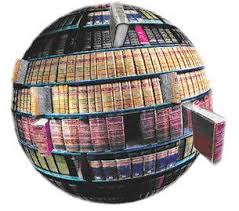
\includegraphics[height=3cm]{Imagenes/repo1}
\end{center}

\end{frame}

\begin{frame}{Gestores de Respositorios}

\begin{itemize}
\item SVN
\item GIT
\item Mercurial
\end{itemize}

\begin{columns}
\column{.4\textwidth}

\includegraphics[height=3cm]{Imagenes/repo_centralizado}
\column{.5\textwidth}
\begin{flushright}
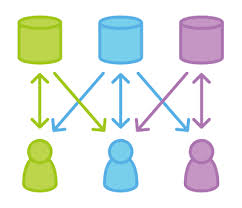
\includegraphics[height=3cm]{Imagenes/repositorio}
\end{flushright}
\end{columns}

\end{frame}


\begin{frame}{Git}

\textbf{Principales caracter�sticas:\\}
\begin{itemize}
\item Sistema de control de versiones distribuido y r�pido.
\item Soporte robusto de branching y merging.
\item Muy flexible y extensible.
\item Fuerte enfoque en la seguridad de la informaci�n, los archivos no se sobreescriben, se agrega al final.
\item Facilita la recuperaci�n ante problemas de disco.
\end{itemize}


%\begin{flushleft}
%\includegraphics[height=3cm]{Imagenes/mercado}
%\end{flushleft}

\end{frame}

\begin{frame}{Sistemas Distribuidos}

\textbf{Un sistema de control de versiones distribuido permite:\\}

\begin{itemize} 
\item Versiones ?offline? (locales).
\item R�pido conjunto de operaciones locales.
\end{itemize}

\textbf{Como consecuencia:\\}

\begin{itemize} 
\item Commits de cambios puntuales.
\item Se puede buscar en el historial localmente.
\item Branching y merging sencillos de implementar sin complicaciones pasando a ser tareas naturales.
\item Permite mejores organizaciones de trabajo (workflows).
\end{itemize}

\begin{center}
		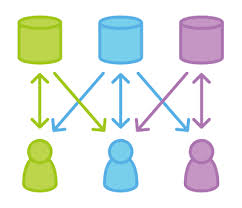
\includegraphics[height=3cm]{Imagenes/repositorio}
\end{center}	

\end{frame}




\begin{frame}{Conceptos}

\begin{flushleft}
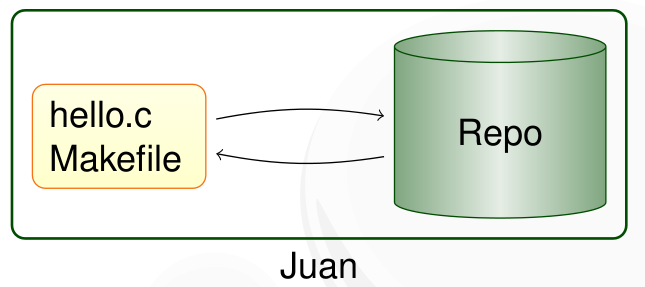
\includegraphics[height=2.95cm]{Imagenes/repo_local}
\end{flushleft}
\begin{itemize}
\item \textbf{Directorio de trabajo:} Es un directorio donde est�n los archivos que queremos administrar.
\item \textbf{Changeset:} Conjunto de cambios en los archivos entre una revisi�n y la siguiente.
\item \textbf{Repositorio:} Guarda el historial de nuestro trabajo (almacena los changesets).
\end{itemize}

\end{frame}

\begin{frame}{Comandos Claves}

\textbf{Locales: }\\
\begin{block}{}
\textbf{git add:} Agrega un cambio al directorio de trabajo.\\
\textbf{git commit:} guarda el estado actual del directorio de trabajo en el repositorio (local).\\
\textbf{git merge:} une distintas l�neas (branches) del historial.
\end{block}

\textbf{Interacci�n con otro repositorio:}\\

\begin{block}{}
\textbf{git clone:} crea un repositorio igual a otro.\\
\textbf{git pull:} trae changesets desde otro repositorio.\\
\textbf{git push:} env�a tus changesets hacia otro repositorio.\\
\end{block}


%\begin{center}
%\includegraphics[height=3cm]{Imagenes/solid_medical2}\\
%\textbf{Modelado 3D}

\end{frame}

\begin{frame}{Modo de Trabajo}

\begin{center}
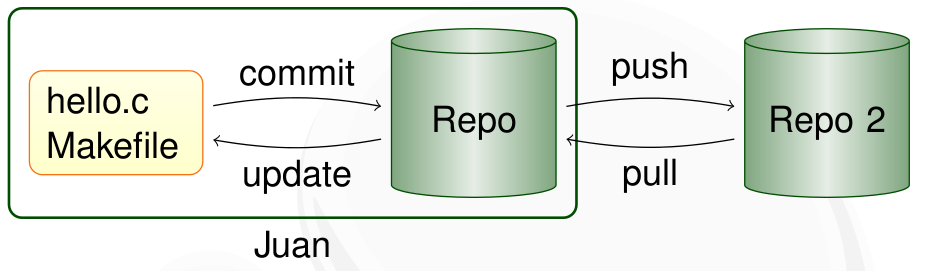
\includegraphics[height=2cm]{Imagenes/repo_modo_trabajo}\\
%\textbf{Proceso de Impresi�n 3D}
\end{center}
\begin{center}
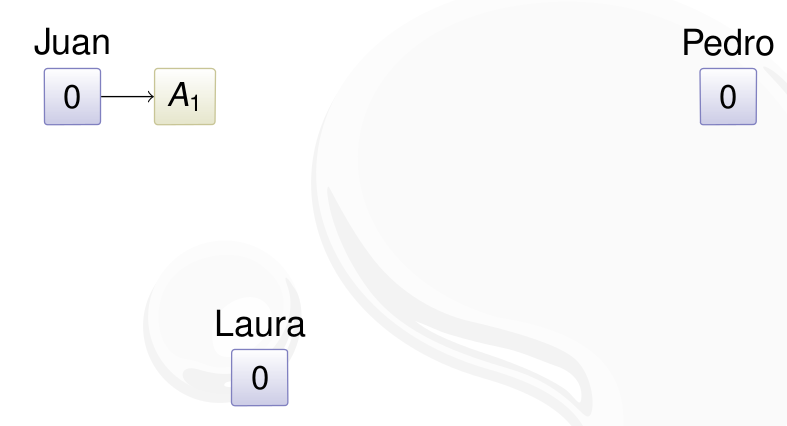
\includegraphics[height=4cm]{Imagenes/repo_changeset1}
%\textbf{Simulaci�n Num�rica}
\end{center}

\end{frame}


\begin{frame}{Modo de Trabajo}
\begin{center}
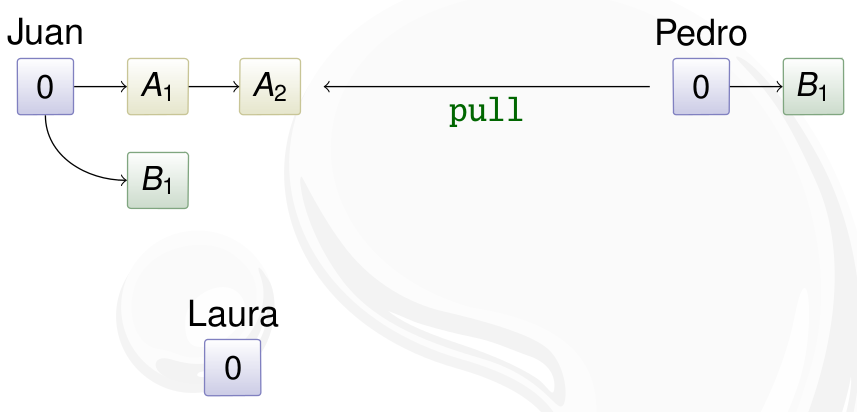
\includegraphics[height=4cm]{Imagenes/repo_changeset4}%\textbf{Simulaci�n Num�rica}
\end{center}
\begin{center}
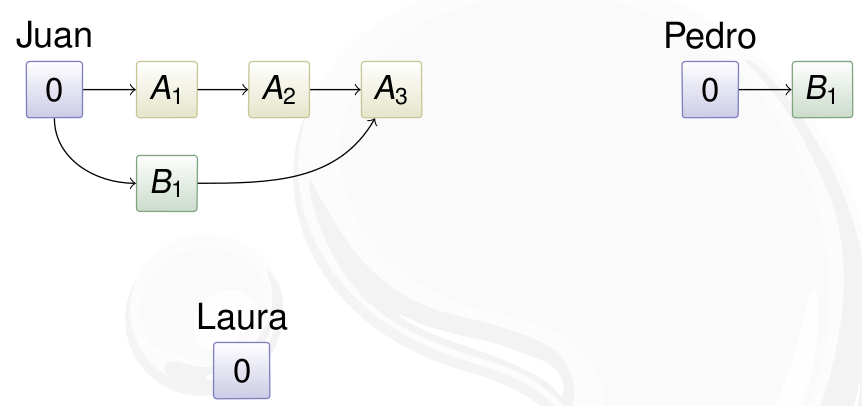
\includegraphics[height=4cm]{Imagenes/repo_changeset5}
%\textbf{Simulaci�n Num�rica}
\end{center}
\end{frame}


\begin{frame}{Modo de Trabajo}
\begin{center}
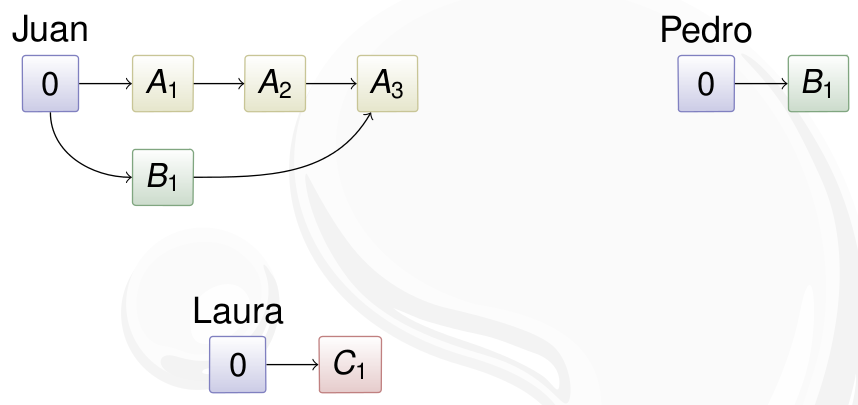
\includegraphics[height=4cm]{Imagenes/repo_changeset6}%\textbf{Simulaci�n Num�rica}
\end{center}
\begin{center}
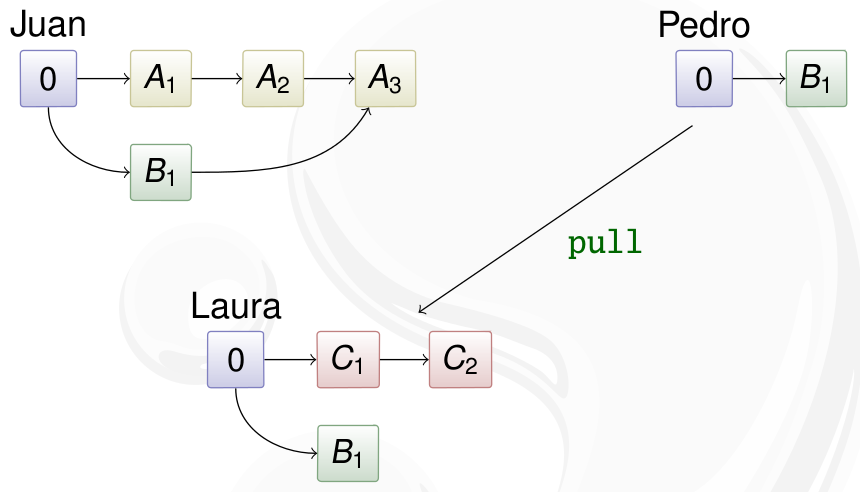
\includegraphics[height=4cm]{Imagenes/repo_changeset7}
%\textbf{Simulaci�n Num�rica}
\end{center}

\end{frame}

\begin{frame}{Modo de Trabajo}

\begin{center}
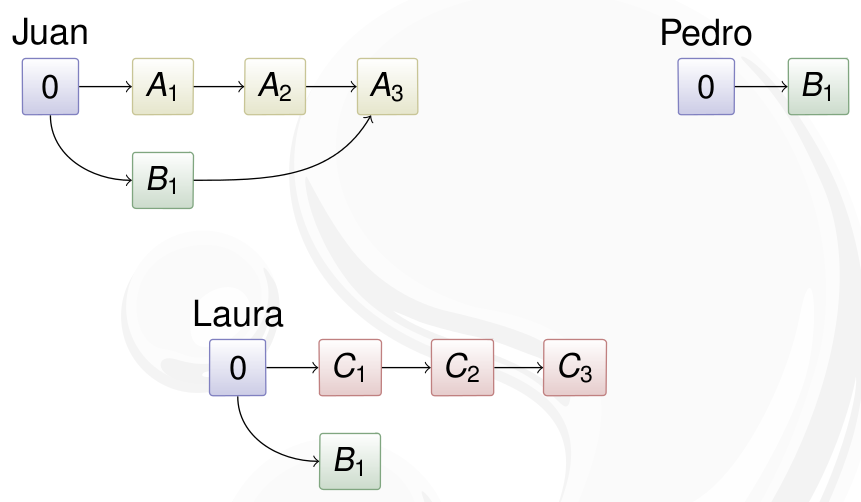
\includegraphics[height=4cm]{Imagenes/repo_changeset8}%\textbf{Simulaci�n Num�rica}
\end{center}
\begin{center}
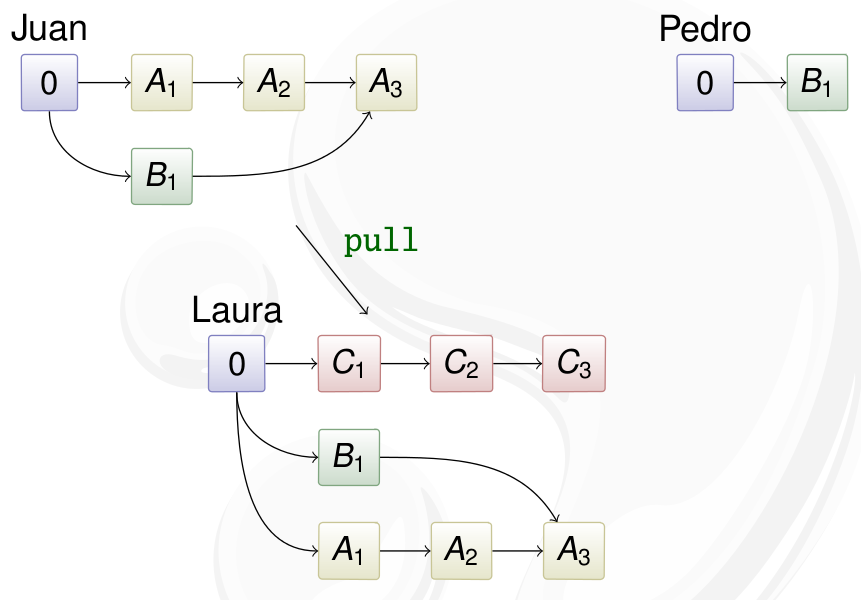
\includegraphics[height=4cm]{Imagenes/repo_changeset9}
%\textbf{Simulaci�n Num�rica}
\end{center}
\end{frame}

\begin{frame}{Modo de Trabajo}
\begin{center}
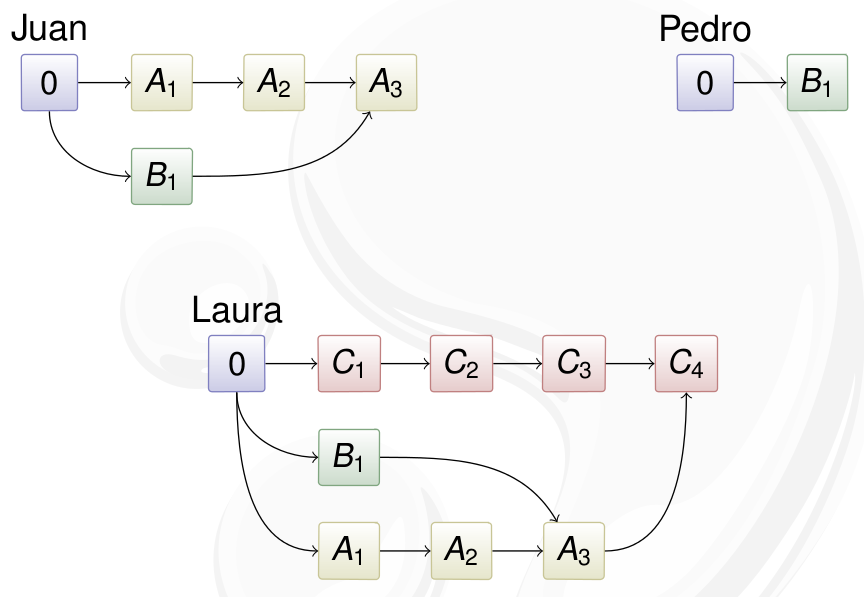
\includegraphics[height=4cm]{Imagenes/repo_changeset10}%\textbf{Simulaci�n Num�rica}
\end{center}
\begin{center}
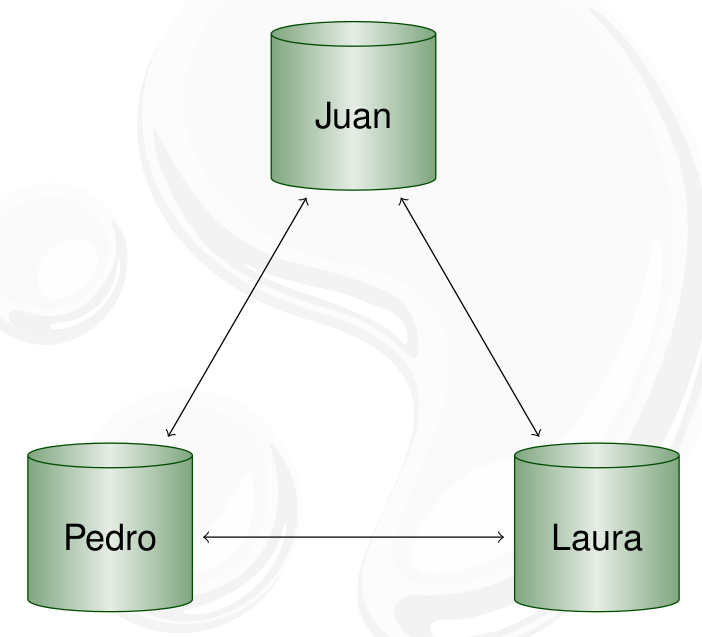
\includegraphics[height=3.2cm]{Imagenes/repo_changeset11}%\textbf{Simulaci�n Num�rica}
\end{center}

\end{frame}

\begin{frame}{Modo de Trabajo}
\begin{center}
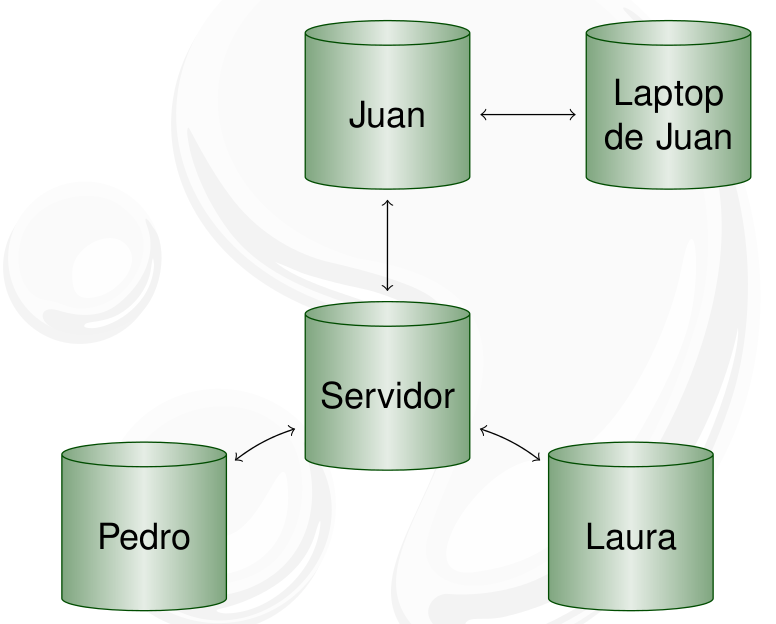
\includegraphics[height=5cm]{Imagenes/repo_changeset13}%\textbf{Simulaci�n Num�rica}
\end{center}

\end{frame}

\begin{frame}{Modo de Trabajo}
\begin{center}
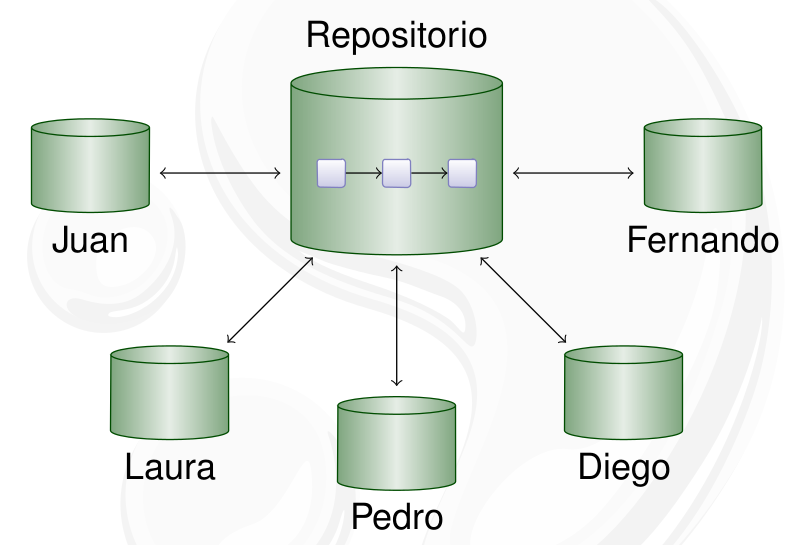
\includegraphics[height=5cm]{Imagenes/repo_changeset14}%\textbf{Simulaci�n Num�rica}
\end{center}

\end{frame}

\begin{frame}{Branches}

Son un concepto clave:\\
L�neas de desarrollo paralelas.\\
Usadas para hacer releases.\\
Usadas para aislar cambios invasivos.\\

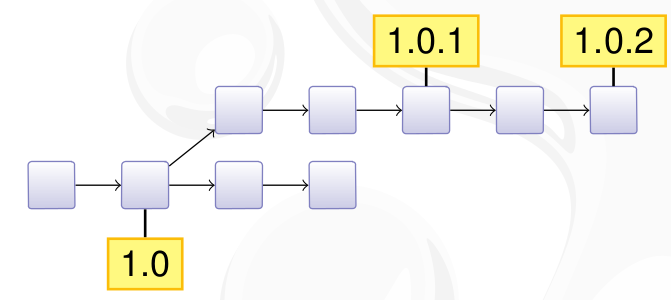
\includegraphics[height=3cm]{Imagenes/repo_branch1}
\end{frame}

\begin{frame}{Merge}

Es lo opuesto al branch:\\
Combina dos branches.\\
Usado para traer arreglos realizados en otros branches.\\
Usado para integrar cambios invasivos una vez
terminados.\\

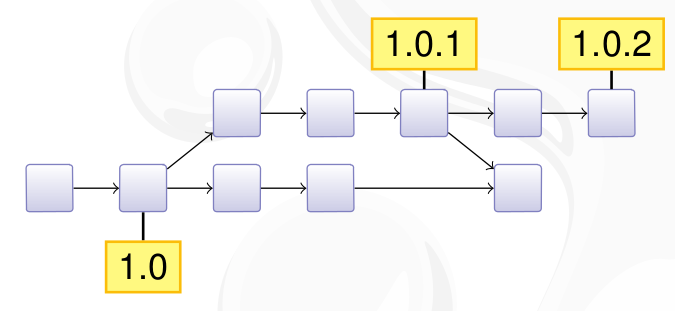
\includegraphics[height=3cm]{Imagenes/repo_merge1}
\end{frame}


\begin{frame}{Desarrollo de Firmware}
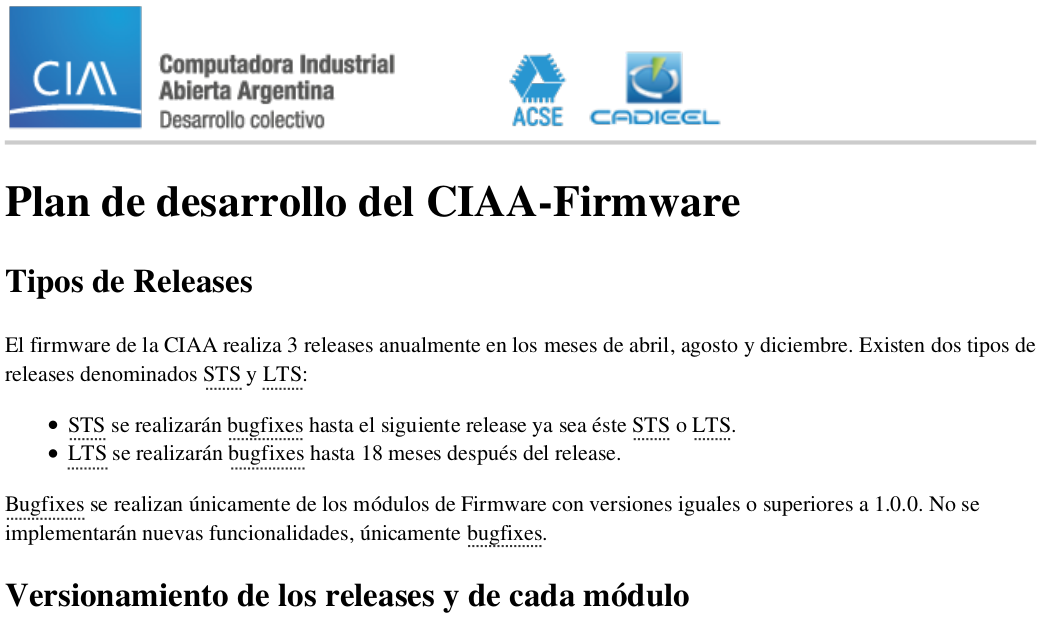
\includegraphics[height=5.5cm]{Imagenes/plan_soft}
\end{frame}

\begin{frame}{Herramienta Libre: GitHub}

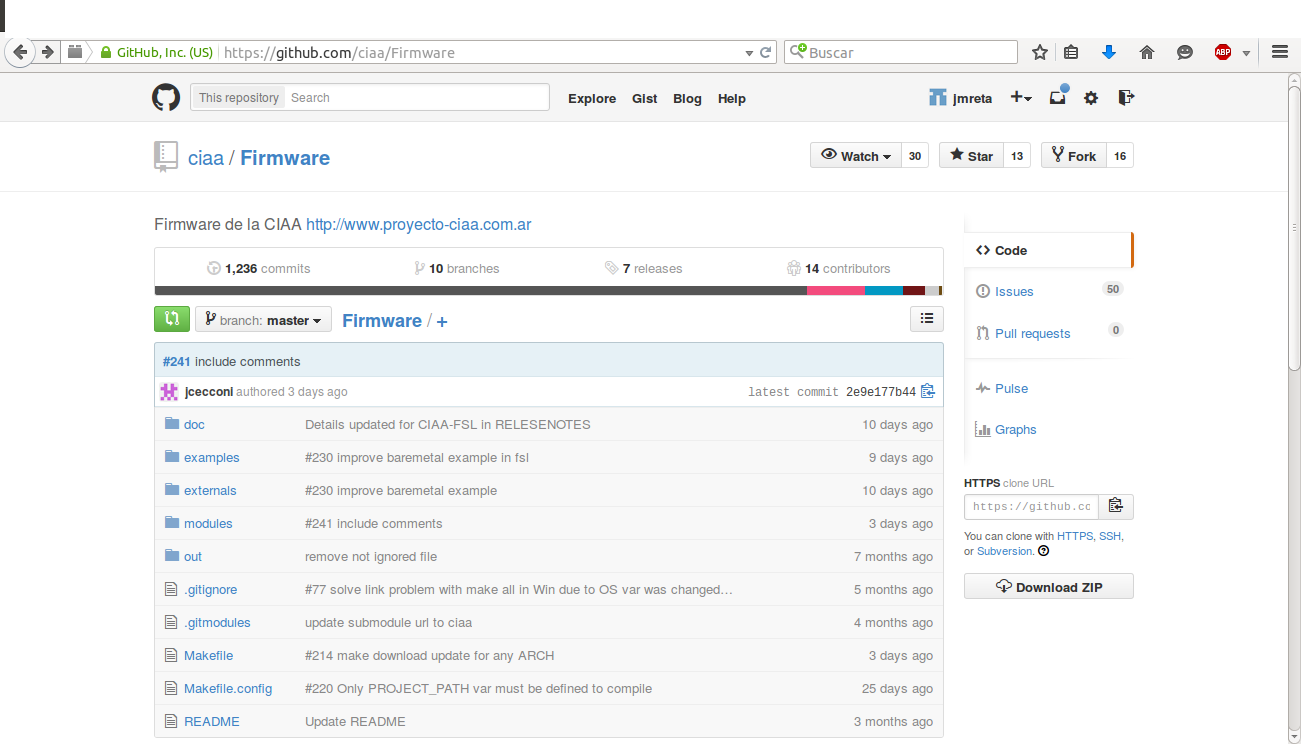
\includegraphics[height=5.5cm]{Imagenes/github}
\end{frame}


\begin{frame}{Estructura Repositorio}

\begin{center}
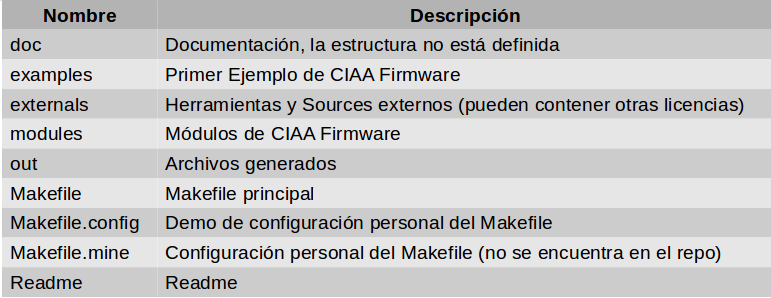
\includegraphics[height=3.5cm]{Imagenes/estructura_repo}
\end{center}
\vspace{0.2 cm}
\begin{center}
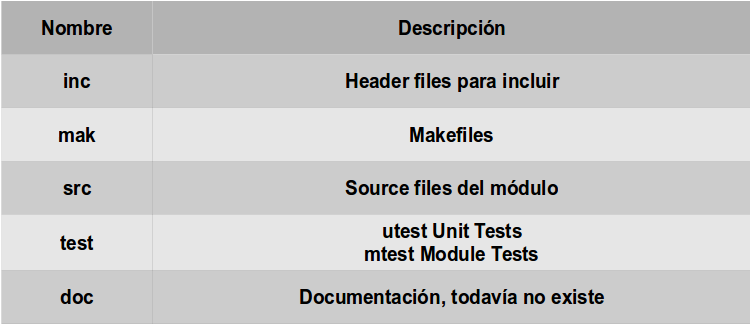
\includegraphics[height=3.5cm]{Imagenes/estructura_modulos}
\end{center}
\end{frame}
\subsection{Estructura Firmware}
\begin{frame}{Estructura Firmware}

\begin{center}
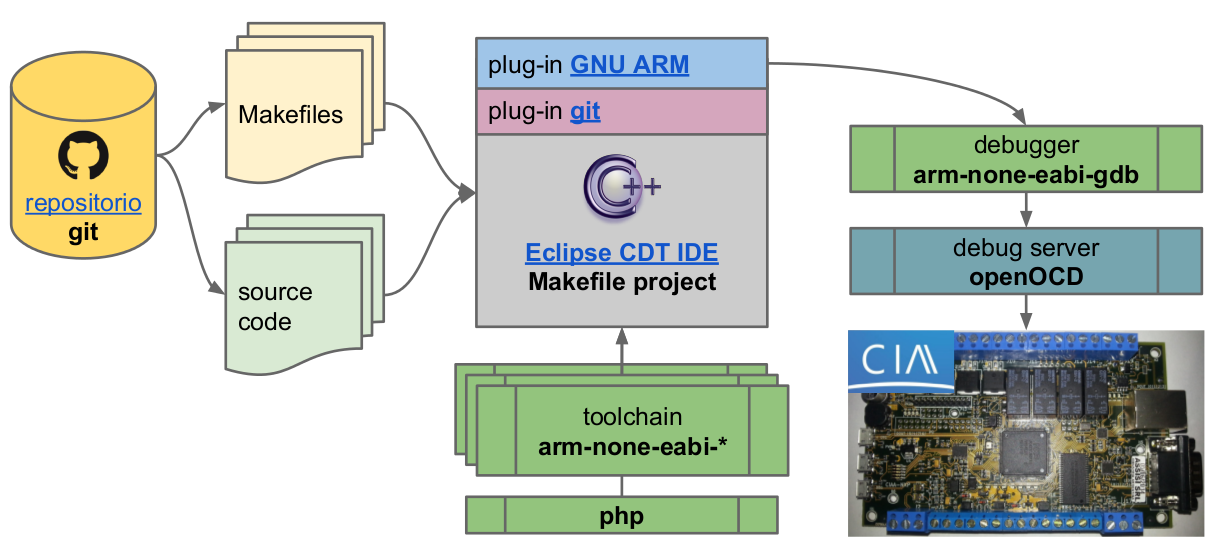
\includegraphics[height=4.5cm]{Imagenes/fimrware}
\end{center}

\end{frame}



\end{document}


